\chapter{Discussion}
\label{sec:discussion}

In this chapter, we explore how competence mapping integrates into the AEM Fiber customer support workflow. We discuss the phases of call creation, update, and ticket processing, explaining how data related to %\textcolor{orange}{maybe is not a matter of "data from" but like \textit{related to }}
these stages help extract communication, technical, and problem-management competences. We also present a straightforward design for a competence mapping dashboard designed to assist HR and management in evaluating departmental and individual performance. This chapter expands on the ideas discussed in Chapter \ref{sec:results}.

\section{Competence mapping integration in case study customer support workflow}

The following is the updated AEM Fiber customer support workflow.

\begin{figure}[ht]
      \centering
      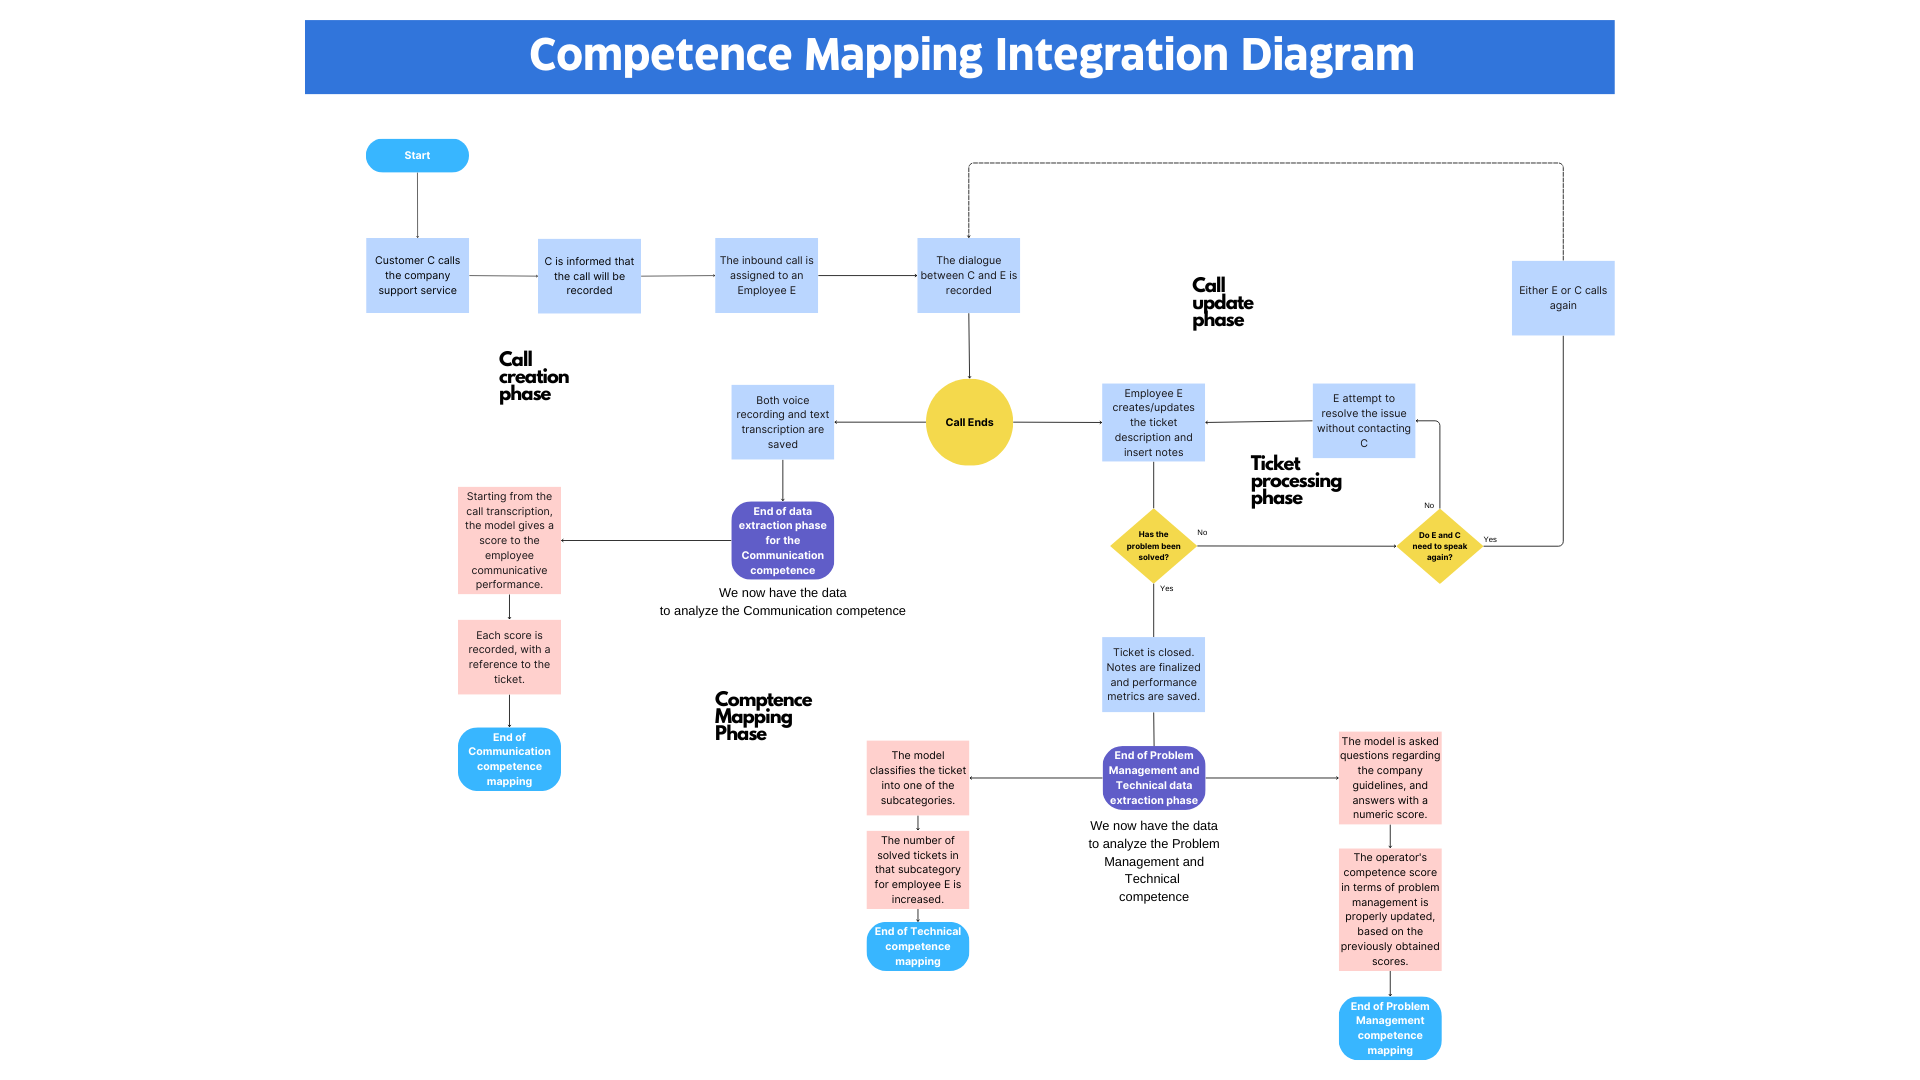
\includegraphics[width=\textwidth]{workflow_integrated.png}
      \caption{Competence mapping updated workflow}
      \label{figure:workflow_integrated}
\end{figure}

\subsection{Call creation phase}

\begin{enumerate}
      \item Customer C calls the company support service to require assistance through the available communication channels.
      \item C is informed that the call will be recorded.
      \item The inbound call is assigned to Employee E.
      \item The dialogue between C and E is recorded.
      \item The call ends.
      \item We have now all the data needed for the communication competence extraction.
\end{enumerate}

\subsection{Call update phase}

\begin{enumerate}
      \item Either Customer C or Employee E calls to provide/require updates on the reported issue.
      \item C is informed that the call will be recorded.
      \item The dialogue between C and E is recorded.
      \item The call ends.
      \item We have now all the data needed for the communication competence extraction.
\end{enumerate}

\subsection{Ticket processing phase}

\begin{enumerate}
      \item At the end of the first call (Call creation phase), employee E creates the ticket description.
      \item If needed the ticket is escalated from level 1 to level 2.
      \item After each operator attempts to solve the issue or after any update call to/from the customer (Call update phase), new working notes are added to the existing ticket.
      \item When the problem has been solved and the customer is satisfied, notes are finalized and the ticket is closed.
      \item At this point, we have all the data needed to extract the Technical and Problem Management competences.
\end{enumerate}

\subsection{Communication competence score extraction}

\begin{enumerate}
      \item Starting from the call transcription, the model gives a score to the employee's communicative performance.
      \item Each score is recorded, with a reference to the ticket.
\end{enumerate}

\subsection{Technical competence score extraction}

\begin{enumerate}
      \item As previously specified, the domain expert has provided a list of the possible subcategories for the ticket categorization, each associated with a difficulty level.
      \item The model classifies the ticket into one of the subcategories.
      \item The number of solved tickets in that subcategory for employee E is increased.
\end{enumerate}

The subcategory difficulty can be useful to understand how well an employee is learning.
We expect that Level 1 employees with longer tenures in the company will be less inclined to escalate simpler tasks to higher levels. The difficulty level can also be useful to compare the proficiency level in different tasks. If the task is considered difficult, a lower score can be considered a good score (e.g. 3.3/4 can be considered very good for a difficult task, but not enough for an easy one).

\subsection{Problem Management score extraction}

\begin{enumerate}
      \item As previously specified, the domain expert has provided a guideline regarding the key points that have to be followed during the problem resolution.
      \item The model is asked questions regarding the provided guideline; each answer corresponds to a certain score.
      \item The operator's competence score in terms of problem management is properly updated, based on the previously obtained scores.
\end{enumerate}

If the ticket has been escalated from level 1 to level 2, only the level 2 employee working notes are taken into consideration while producing the problem management score.

\section{Possible design of the competence mapping dashboard}

To better support HR and higher-level management, we've introduced a straightforward performance dashboard. Here, managers can access both general department metrics and specific details for individual employees. The left side of the dashboard displays competence evaluations for each employee. On the right, managers can compare employees using scatterplots based on various KPIs. This comparison aids in identifying high-performing employees for potential promotion and those needing additional training, as can be seen in Figure \ref{figure:recap}. Clicking on an employee's name reveals a detailed view, summarizing overall performance and listing the most recent assigned tickets. Managers can further analyze each competence by clicking the detail button, as shown in Figure \ref{figure:employee_overall}. Within the detailed competence view, sub-competences are broken down for a closer look. For instance, the communication competence is presented with graphs detailing specific strengths and areas for improvement. This straightforward approach equips managers with the necessary insights for departmental and individual performance assessments, as detailed in Figure \ref{figure:employee_detail}.

\vfill

\begin{figure}[ht]
      \centering
      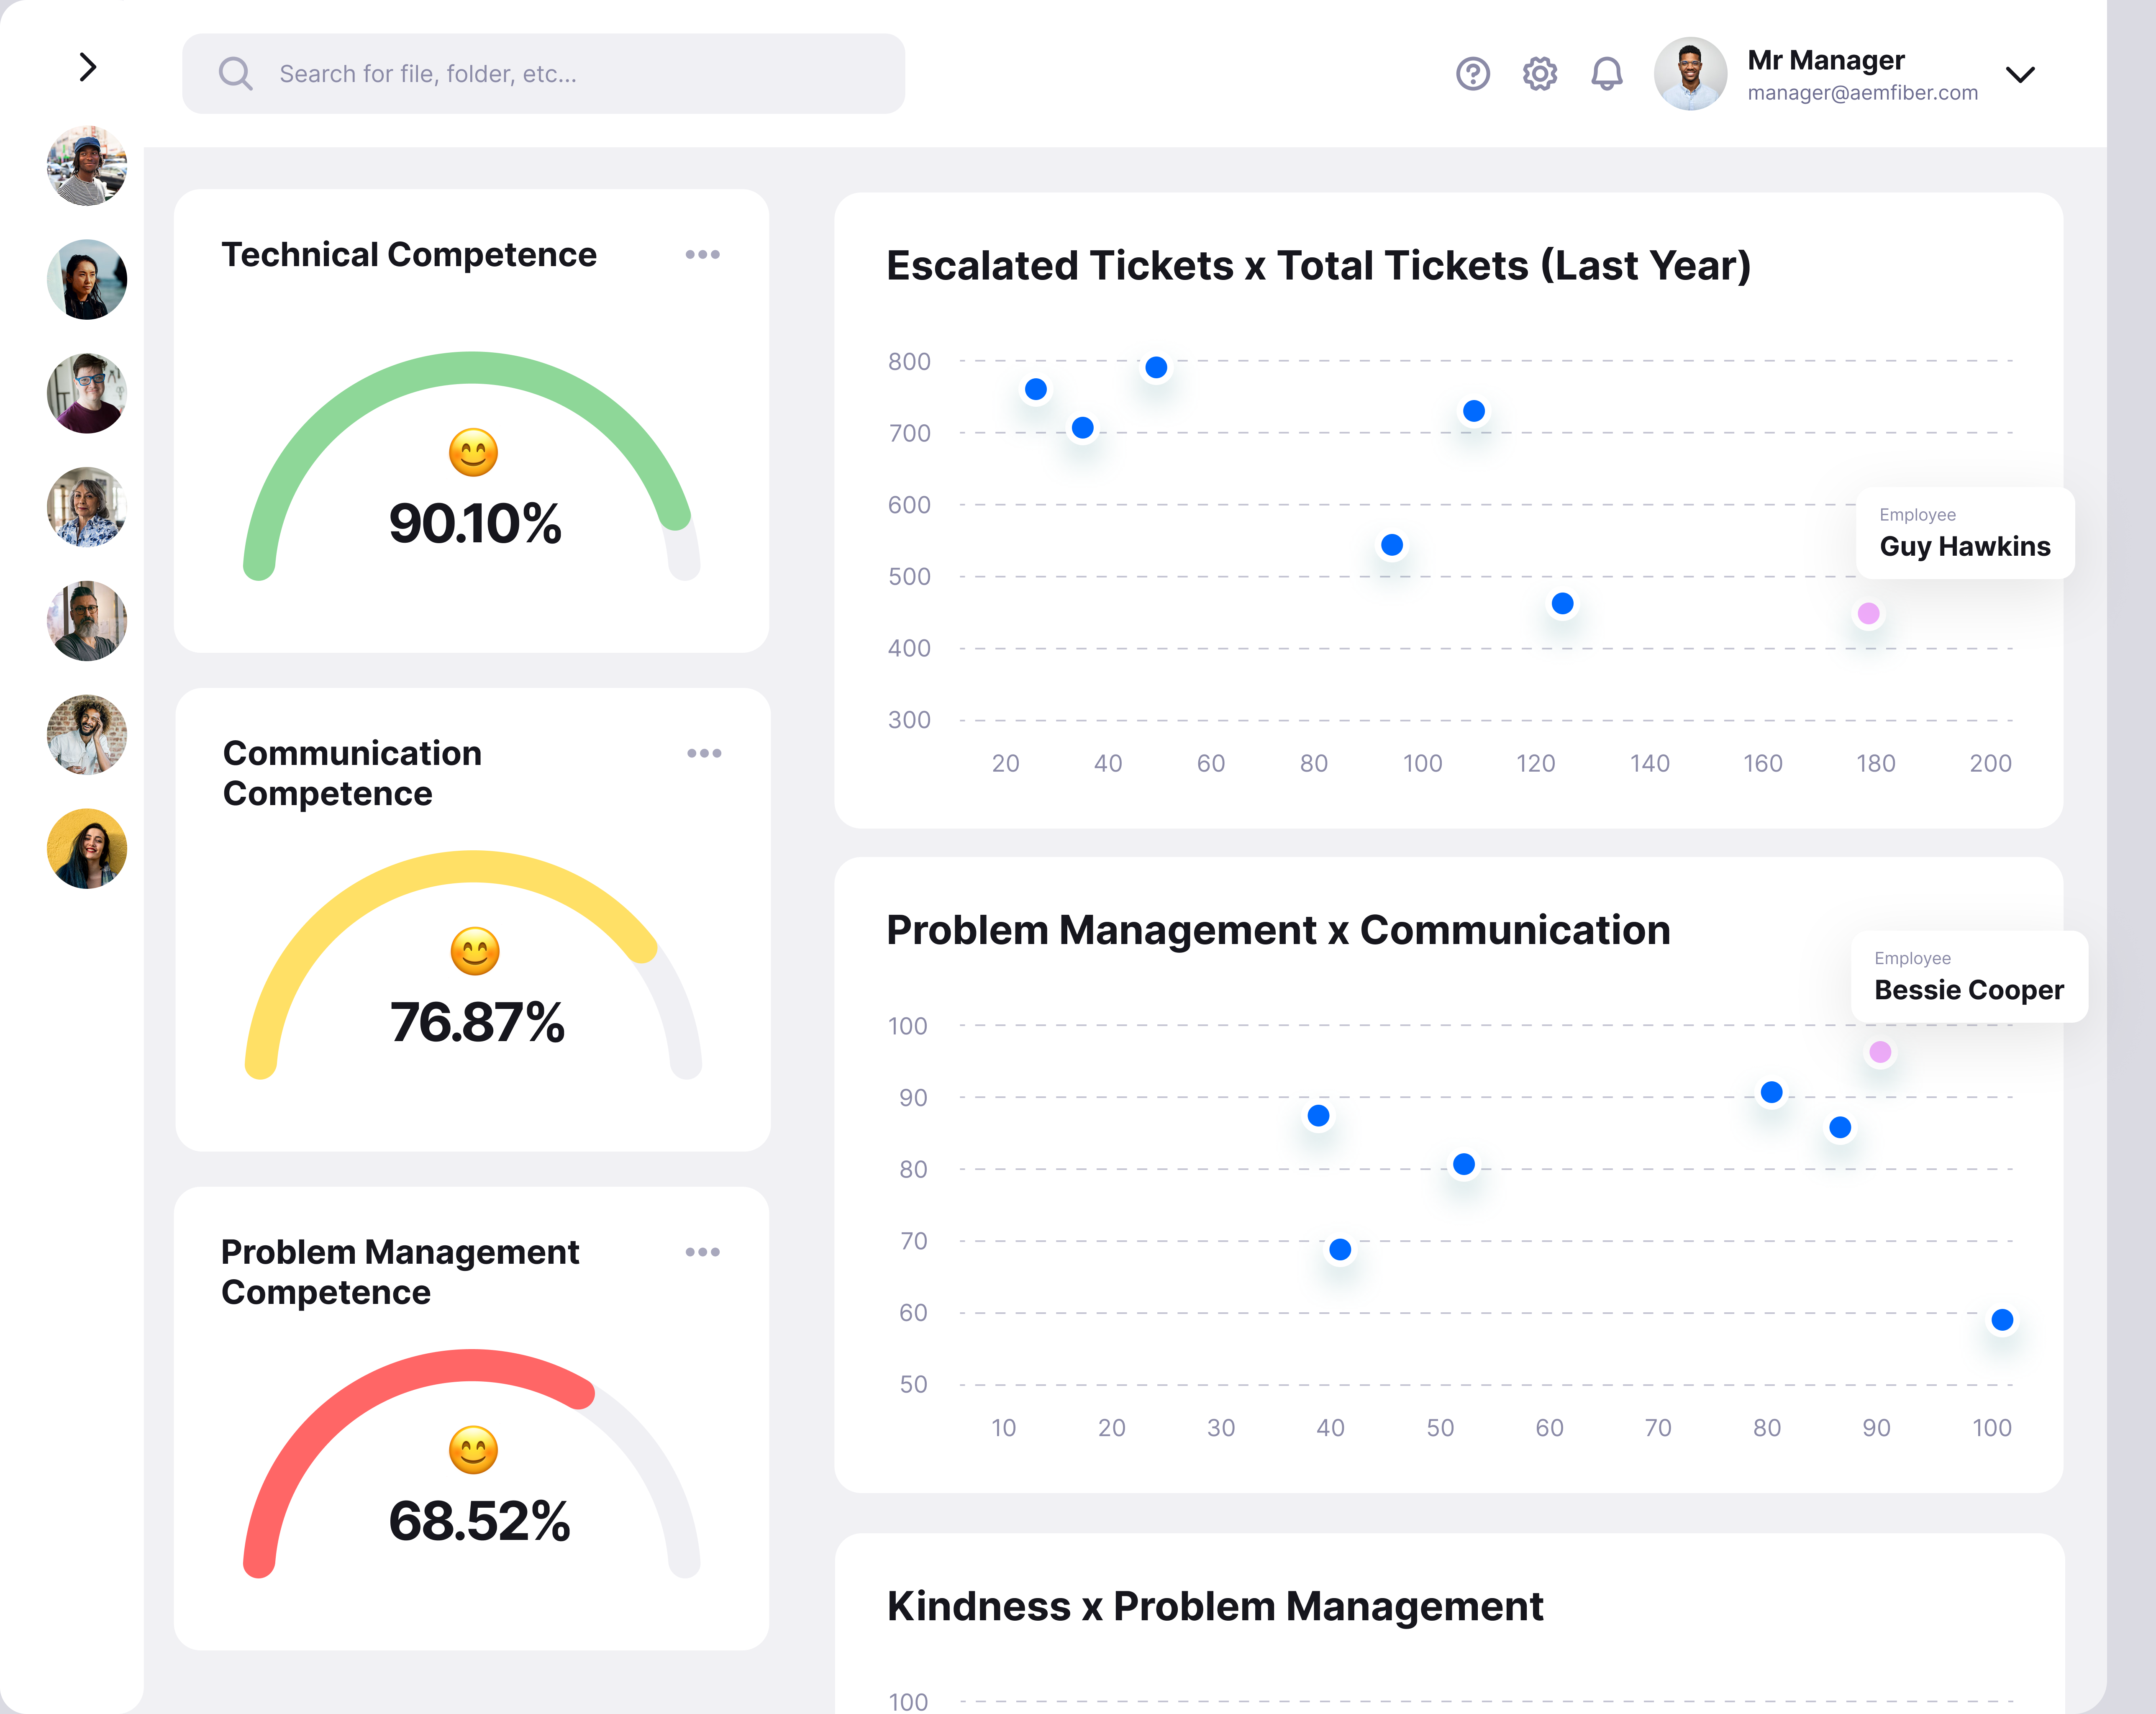
\includegraphics[width=\textwidth]{recap.png}
      \caption{Dashboard performance recap mock-up}
      \label{figure:recap}
\end{figure}

\vfill

\begin{figure}[ht]
      \centering
      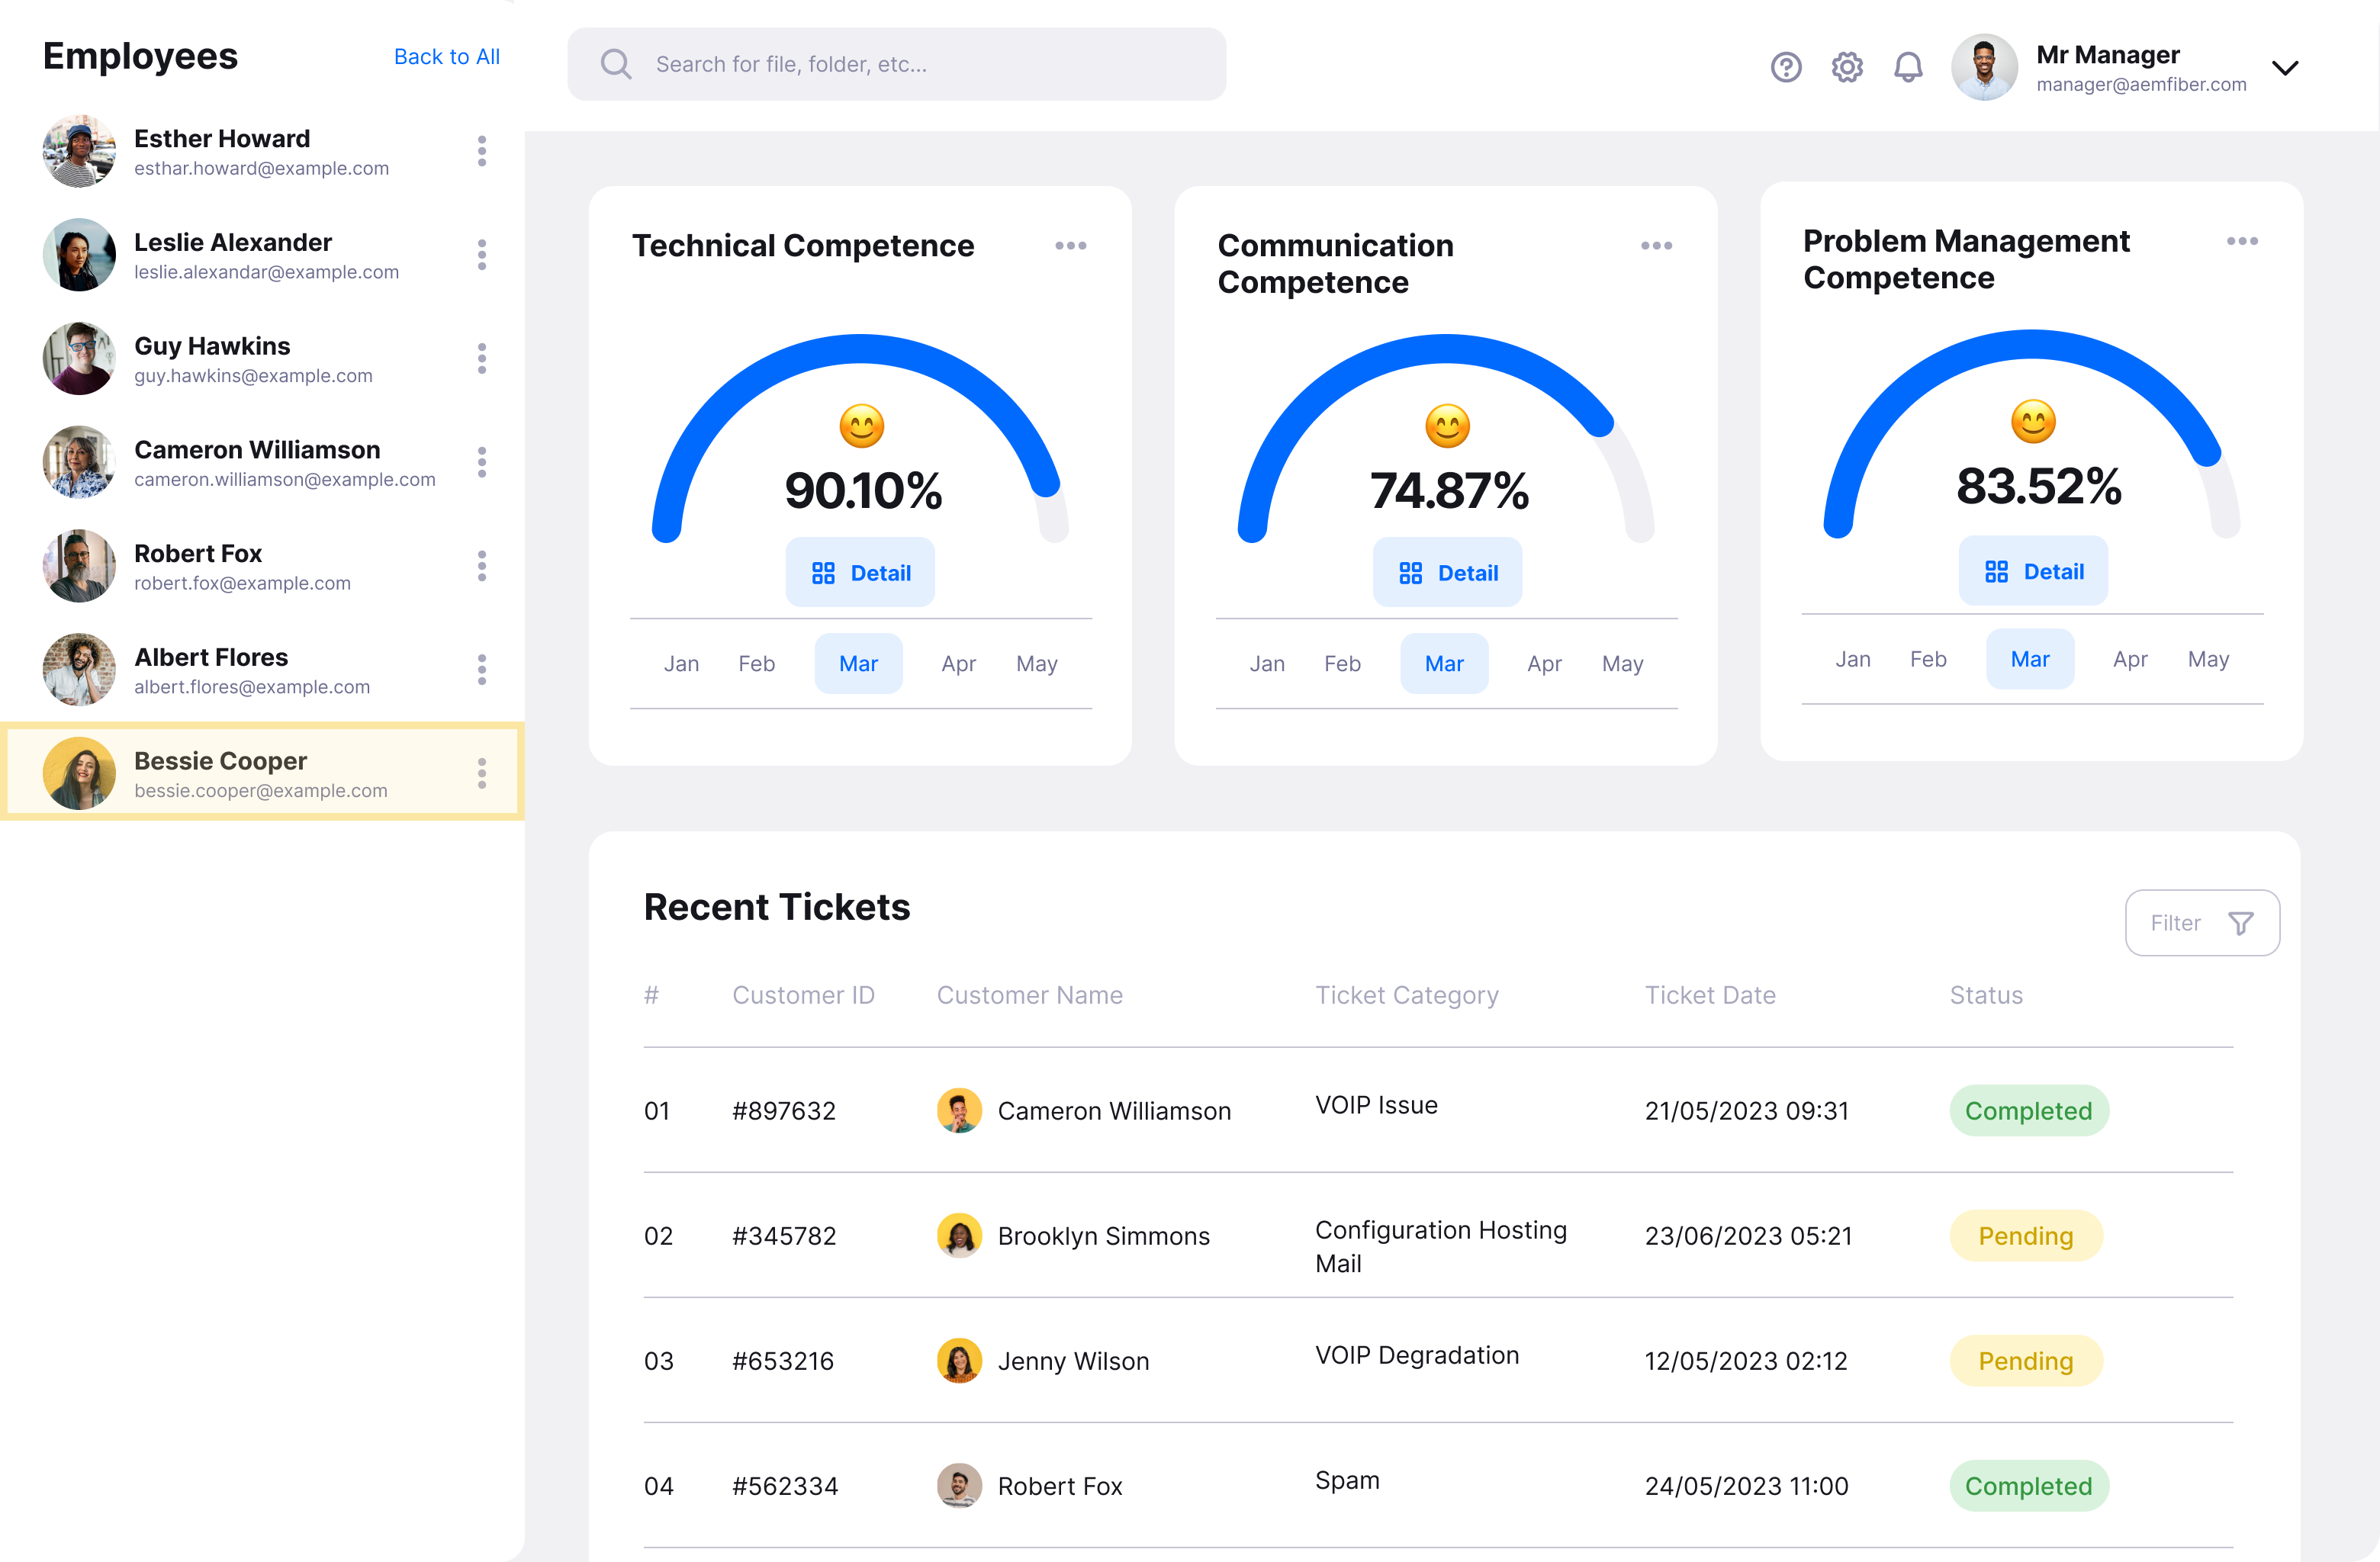
\includegraphics[width=\textwidth]{employee overall.png}
      \caption{Dashboard employee performances mock-up}
      \label{figure:employee_overall}
\end{figure}
\begin{figure}[ht]
      \centering
      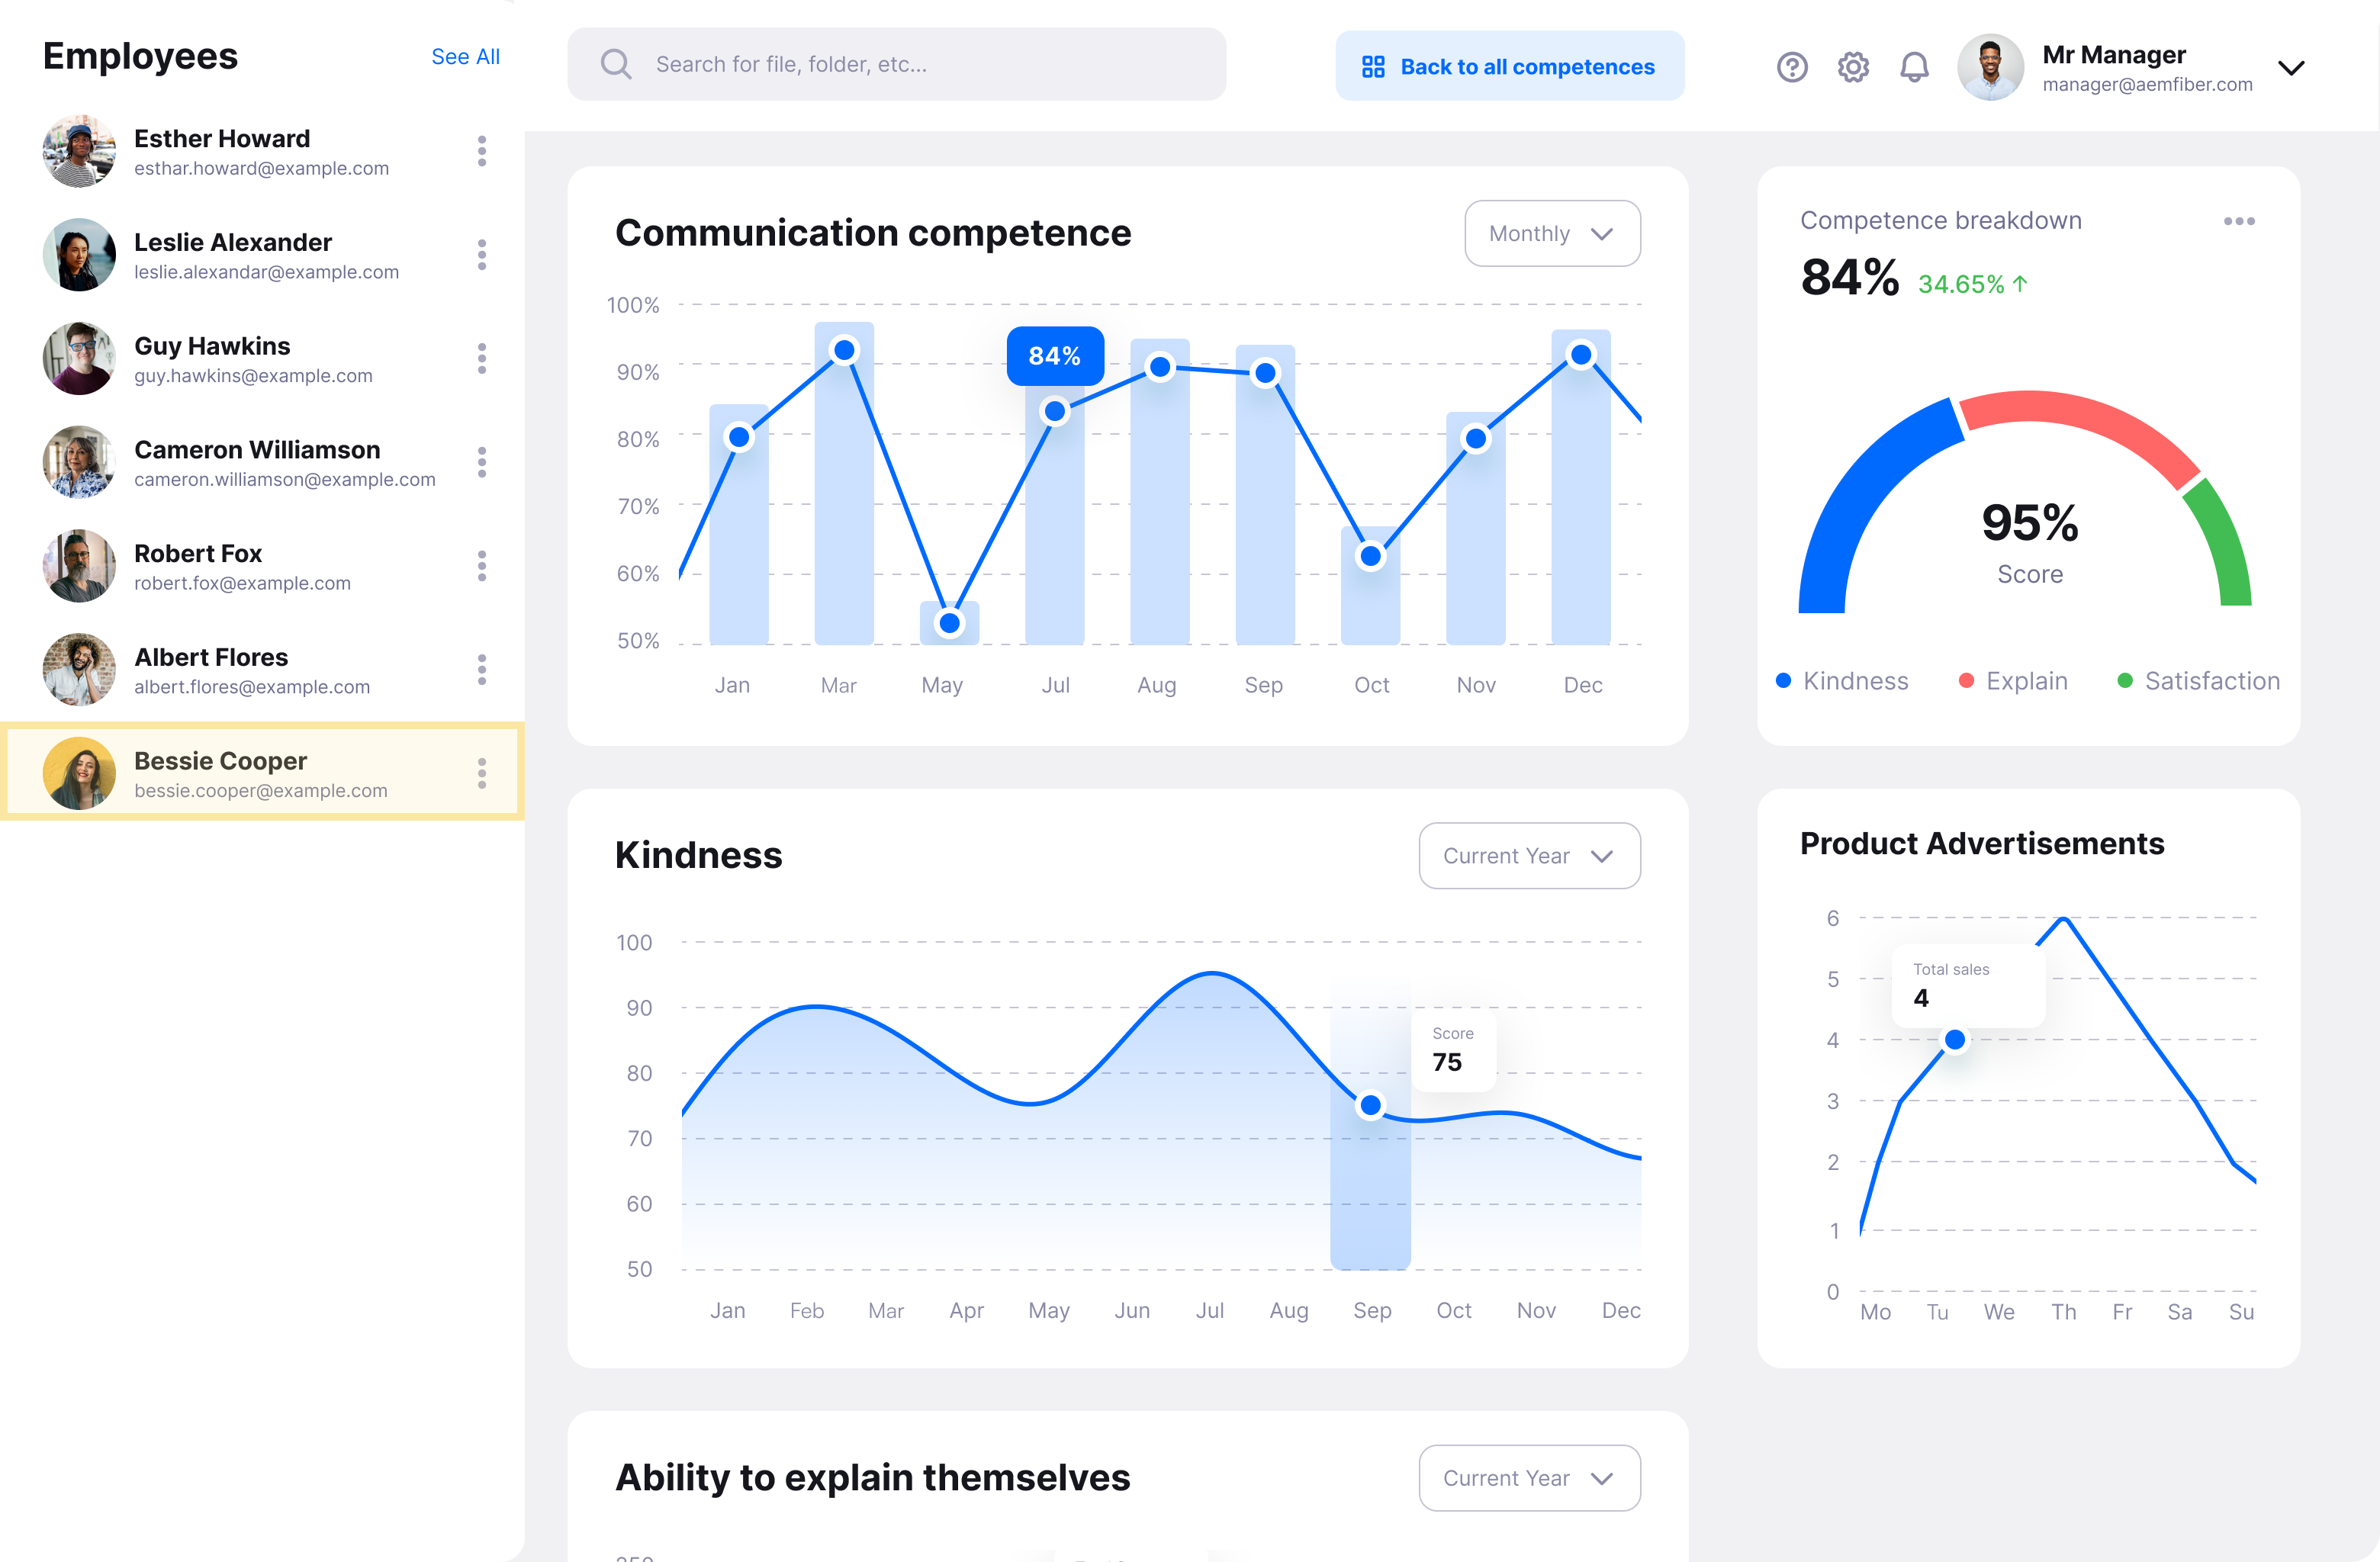
\includegraphics[width=\textwidth]{employee detail.png}
      \caption{Dashboard employee detail mock-up}
      \label{figure:employee_detail}
\end{figure}